\documentclass[twocolumn,journal]{IEEEtran}
\usepackage{amsmath,amsfonts}
% \usepackage{appendix}
\usepackage{amsthm,lipsum}
\usepackage{algorithm,algorithmic}
\usepackage{array}
\usepackage{bm}
\usepackage[font=normalsize]{subfig}
\usepackage{textcomp}
\usepackage{stfloats}
\usepackage{url}
\usepackage{verbatim}
\usepackage{graphicx}
\usepackage[backend=bibtex,sorting=none,style=ieee]{biblatex}
\renewcommand{\bibfont}{\footnotesize}
\addbibresource{refYunbo}
\hyphenation{op-tical net-works semi-conduc-tor IEEE-Xplore}
\def\BibTeX{{\rm B\kern-.05em{\sc i\kern-.025em b}\kern-.08em
    T\kern-.1667em\lower.7ex\hbox{E}\kern-.125emX}}
\usepackage{balance}
\usepackage{xcolor}
\usepackage{tcolorbox}
% \newtheorem{assumption}{\textbf{Assumption}}
\newtheorem{theorem}{\textbf{Theorem}}
% \newtheorem{proof}{\textbf{Proof}}
% \newtheorem{definition}{\textbf{Definition}}
% \newtheorem{proposition}{\textbf{Proposition}}
% \newtheorem{corollary}{\textbf{Corollary}}
% \newtheorem{remark}{\textbf{Remark}}
% \newtheorem{lemma}{\textbf{Lemma}}
\tcbuselibrary{theorems}
% 定义 remark 环境
\newtheorem{remark}{Remark}

\begin{document}
\title{Beamforming and Deployment Design for Cooperative AAV-enabled ISAC with Rate-Splitting Multiple Access under Imperfect CSI}
\author{Yunbo Hu
\thanks{Corresponding author: Liang Tang}}

\markboth{Journal of \LaTeX\ Class Files,~Vol.~18, No.~9, September~2020}%
{How to Use the IEEEtran \LaTeX \ Templates}

\maketitle

\begin{abstract}
In this paper, 
\end{abstract}

\begin{IEEEkeywords}
Integrated sensing and communication (ISAC), robust optimization, autonomous aerial vehicle (AAV)
\end{IEEEkeywords}


\section{Introduction}
Autonomous aerial vehicle (AAV) is commonly considered as an effective platform to provide seamless coverage and enhance the overall performance of celluar networks. The flexible deployment deployment and high mobility of AAV can be utilized to improve the line-of-sight (LoS) channel quality \cite{zengWireless2016}. Moreover, AAV can also be adopted as a suitable sensing platform with relative sensors equipped. The sensing coverage and high perspective view enables AAV to perform remote sensing, mapping, and monitoring tasks \cite{muUAV2023}. Since AAV can be utilized for both communication and sensing, it is natural to integrate these two functionalities on AAV platform, which is referred to as AAV-enabled integrated sensing and communication (ISAC). Such integration can not only enhance the spectrum efficincy, but also enables the hardware reuse to reduce the size, weight, and power (SWaP) consumption of AAV \cite{mengUAVEnabled2024}. Moreover, AAV can exploit the mutual benefits between communication and sensing, i.e., sensing-assisted communication \cite{huCollaborative2025}. 
% due to the hardware constraint of AAV, the full-duplex operation is difficult to implement. Thus, the bistatic/multistatic sensing mode is more suitable for AAV-enabled ISAC system\cite{zhangOverview2021}.

Despite the fact that AAV-enabled ISAC has many advantages, there are still several challenges to tackle. Firstly, an efficient waveform design scheme is required to fully exploit the time and frequence resourse for both communication and sensing \cite{chenJoint2023b}. Thus, suitable joint sensing and communication scheme should be dedicatedly designed. Secondly, the trade-off between sensing and communication should be considered to simultaneously guarantee the performance of both function. For instance, the AAV position has distinct impact on communication and sensing performance respctively \cite{huCollaborative2025}. Therefore, the resourse allocation and AAV deployment should be optimized to balance the performance trade-off. 
Thirdly, the dynamic characteritic of AAV makes the accurate instantaneous channel state information (CSI) aquisition difficult. Since the communication resourse allocation heavily rely on accurate CSI, imperfect CSI should be considered in the AAV-enabled ISAC system \cite{maoUAVAssisted2025}.

Some researches have focused on the AAV-enabled ISAC system and its relative challenges. To design a sensing and communication waveform, in \cite{xuRateSplitting2021a}, researchers study the cooperative localization system based on multiple communication base stations (BSs). Rate-splitting multiple access (RSMA) technology is adopted to flexibly manage the multi-user interference and duplex of sensing and communication. Meanwhile, to solve the resourse allocation problem, researchers in \cite{mengUAVEnabled2023} and \cite{jingISAC2024} investigate the joint trajectory design and resourse allocation method for AAV-enabled monostatic ISAC system. Moreover, to tackle the imperfect CSI issue, a robust beamforming design is proposed in \cite{lyuDualRobust2024} to simultaneously optimize the channel capacity and sensing beam pattern under imperfect CSI. However, the aforementioned works mainly focus on the monostatic sensing mode, which is difficult to implement in AAV-enabled ISAC system due to the hardware constraint of AAV. Thus, bistatic/multistatic framework is more suitable for AAV-enabled ISAC. Nevertheless, due to the fact that the communication symbols are unkonwn to the receivers, the joint sensing and communication scheme should be re-designed, and sensing metrics, such as signal-to-inteference-plus-noise ratio (SINR), should be redefined. Furthermore, the new bistatic/multistatic scheme and sensing metric will induce distinct optimization problem, which should be carefully investigated. 

In this letter, we propose a novel cooperative AAV-enabled ISAC framework, where AAVs transmit the ISAC signals to the user equipments (UEs) and the ground target, and the ground BS receives the echo signals reflected from the target for positioning. To fully exploit the spectrum resourse, three-layer RSMA is adopted to jointly manage the inteference among multi-user and between sensing and communication. Based on the proposed system framework, we model the channel capacity and Cramér-Rao bound (CRB) under the imperfect CSI, and formulate the joint beamforming and AAV deployment optimization problem, which is challenging to solve due to the statistic and non-convexity form of the channel capacity and CRB. To address the the intractable original problem, we propose an effective solution based on alternative optimization (AO) and some equivalent mathmatical transformations. Simulations are conducted to show the advantage of our proposed scheme in both sensing and communication.

\section{System Model}
\begin{figure}[t]
    \centering
    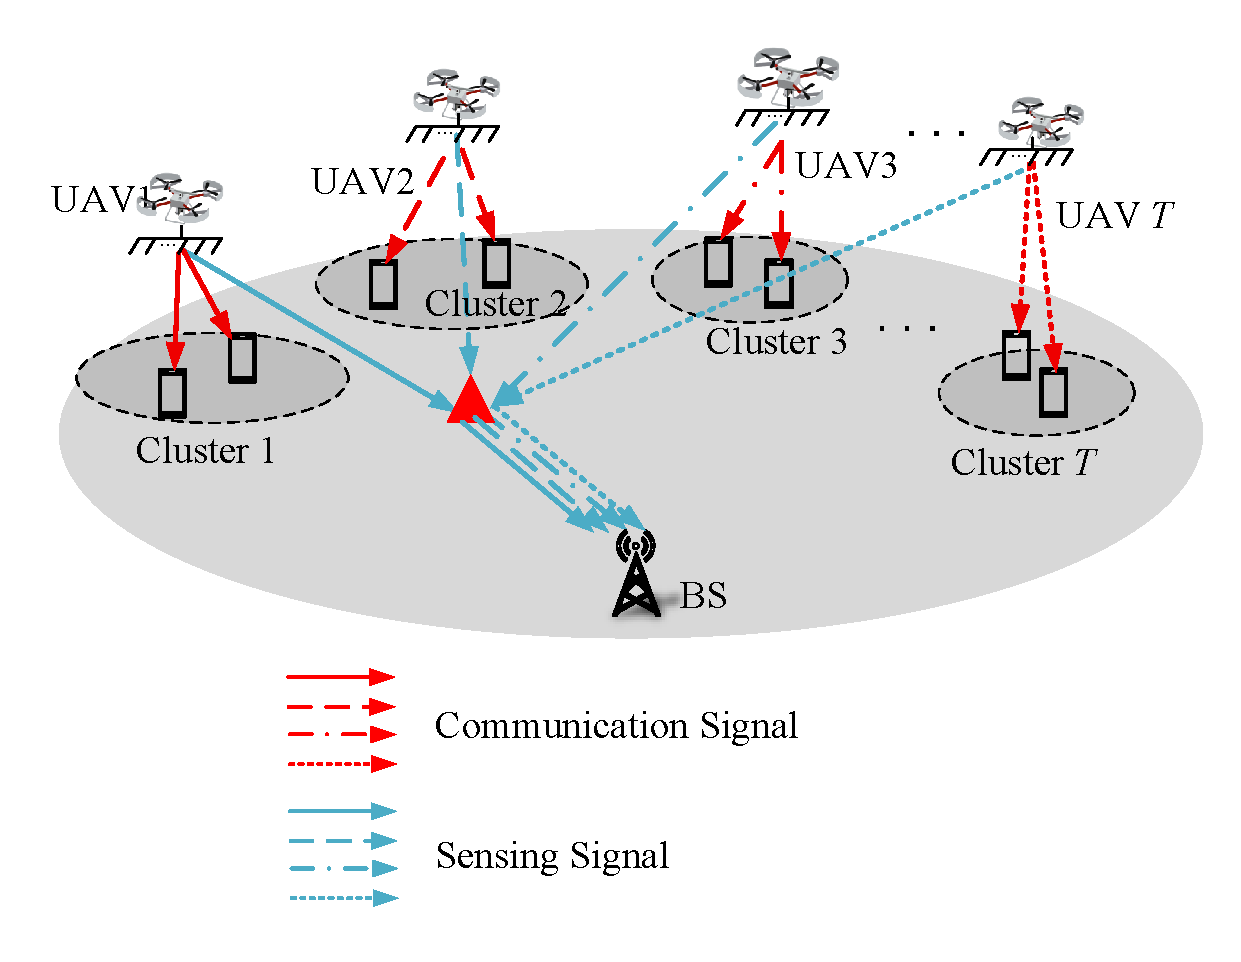
\includegraphics[width = 0.99\linewidth]{figure/systemmodel.pdf}
    \caption{An illustration of the cooperative AAV-enabled ISAC system.}
    \label{fig:systemModel}
\end{figure}
In this section, we focus on a cooperative AAV-enabled ISAC system, which is illustrated in Fig. \ref{fig:systemModel}. There are \(T\) AAVs employed in the serving area, and the UEs are divided into \(T\) clusters served by corresponding AAVs respectively. Without loss of generality, we assume that the number of UE in each cluater is \(K\). Each AAV is equipped with a half-wavelength uniform linear array with \(N_t\) antennas, while each UE is euipped with a single antenna. The AAVs transmit orthogonal ISAC (i.e. time orthogonal or frequency orthogonal) signals to the UEs and the sensing target, and the ground BS with single antenna receives the relected signals from the target for positioning. The coordinates of the \(t\)-th AAV, the \(k\)-th UE in the \(t\)-th cluster, the target, and the ground base station are denoted as \(\boldsymbol{x}^{U}_{t}\), \(\boldsymbol{x}_{t,k}\), \(\boldsymbol{x}_{r}\) and \(\boldsymbol{x}^{B}\in \mathbb{R}^{3\times 1}\), respectively.

\subsection{Signal Model}
Inspired by RSMA, sensing and communication waveform can be emerged non-orthogonally. The received signal of the \(k\)-th UE in the \(t\)-th cluster can be expressed as 
\begin{align}
    y_{t,k} = \boldsymbol{h}^{H}_{t,k}\boldsymbol{p}^{r}_{t} {s}^{r}_{t} + \boldsymbol{h}^{H}_{t,k}\boldsymbol{p}^{c}_{t}{s}^{c}_{t} + \boldsymbol{h}^{H}_{t,k}\sum_{k=1}^{K} \boldsymbol{p}^{p}_{t,k} {s}^{p}_{t,k} + n_{t,k},
\end{align}
where \(s^{r}_{t}\), \(s_{t}^{c}\), and \(s^{p}_{t,k}\) denote the radar sequence, the common message, and the private message for the \(k\)-th UE in the \(t\)-th cluster, respectively. And we assume that \(\mathbb{E}(s^{r}_{t})=\mathbb{E}(s_{t}^{c})=\mathbb{E}(s^{p}_{t,k})=1\). \(\boldsymbol{p}^{r}_{t}\), \(\boldsymbol{p}^{c}_{t}\), and \(\boldsymbol{p}^{p}_{t,k}\in\mathbb{C}^{N_t\times 1}\) denote the corresponding precoding vectors. \(n_{t,k}\) denotes the Gaussian white noise, which follows the distribution of \(\mathcal{CN}(0,\sigma^2)\). \(\boldsymbol{h}_{t,k}\in\mathbb{C}^{N_t \times 1}\) dentes the channel vector between the \(t\)-th AAV and the \(k\)-th UE in the \(t\)-th cluster. Considering the channel uncertainty, the estimated channel \(\hat{\boldsymbol{h}}_{t,k}\) satisfies 
\begin{align}
    \boldsymbol{h}_{t,k} = \hat{\boldsymbol{h}}_{t,k} + \Delta\boldsymbol{h}_{t,k}, \forall k,t,\label{eq:commChannelUncertainty}
\end{align} 
where \(\Delta\boldsymbol{h}_{t,k}\) denotes the channel estimation error jointly caused by the AAV jitter and noise, and \(\hat{\boldsymbol{h}}_{t,k}\) denotes the imperfect CSI at the \(k\)-th AAV. \(\hat{\boldsymbol{h}}_{t,k}\) is related to the position of the \(t\)-th AAV and \(k\)-th UE, which can be modeled as \cite{linMultiAntenna2024}
\begin{align}
    \hat{\boldsymbol{h}}_{t,k} = \sqrt{\frac{\beta}{\left\Vert \boldsymbol{x}^{U}_{t} - \boldsymbol{x}_{t,k} \right\Vert^2}}\boldsymbol{a}(\theta_{t,k}),
\end{align}
where \(\beta\) denotes the channel gain at the reference distance of \(1;\text{m}\), the steering vector \(\boldsymbol{a}(\theta_{t,k})\) is defined as \(\boldsymbol{a}(\theta_{t,k})=[1,\exp(-j\pi\sin\theta_{t,k}),\cdots,\exp(-j\pi\sin\theta_{t,k}(N_t-1))]^H\), and \(\theta_{t,k}\) denotes the angle of departure (AoD) between the \(t\)-th AAV and the \(k\)-th UE. Without generality, we assume that the ULA is parallel to the \(x\)-axis, thus \(\sin\theta_{t,k} = \frac{\boldsymbol{x}^{U}_{t}(2) - \boldsymbol{x}_{t,k}(2)}{\Vert \boldsymbol{x}^{U}_{t} - \boldsymbol{x}_{t,k}\Vert}\).

The CSI error is assumed to be bounded \cite{xuResource2025}, i.e., \(\|\Delta\boldsymbol{h}_{t,k}\| \leq \epsilon_{c,t,k}\), where \(\epsilon\) denotes the maximum channel estimation error. 

Similarly, the received signal from the \(k\)-th AAV at the ground BS can be written as 
\begin{align}
    r_k = \boldsymbol{g}^{H}_{k}\boldsymbol{p}^{r}_{k} {s}^{r}_{k} + \boldsymbol{g}^{H}_{k}\boldsymbol{p}^{c}_{k}{s}^{c}_{k} + \boldsymbol{g}^{H}_{k}\sum_{k=1}^{K} \boldsymbol{p}^{p}_{k,k} {s}^{p}_{k,k} + w_k,
\end{align}
where \(w_k\) denotes the Gaussian white noise, which follows the distribution of \(\mathcal{CN}(0,\sigma^2)\). \(\boldsymbol{g}_{k}\in\mathbb{C}^{N_t \times 1}\) denotes the channel vector between the \(k\)-th AAV and the ground BS. The real channel \(\hat{\boldsymbol{g}}_{k}\) satisfies
\begin{align}
     \boldsymbol{g}_{k} = \hat{\boldsymbol{g}}_{k} + \Delta\boldsymbol{g}_{k}, \forall k,t,\label{eq:sensingChannelUncertainty}
\end{align} 
where the sensing channel error \(\Delta\boldsymbol{g}_{k}\) also satisfies the bounded model \(\|\Delta\boldsymbol{g}_{k}\| \leq \epsilon_{r,k}\), and the imperfect sensing CSI \(\hat{\boldsymbol{g}}_{k}\) can be modeled as
\begin{align}
    \hat{\boldsymbol{g}}_{k} = \sqrt{\frac{\beta \sigma_r}{\left\Vert \boldsymbol{x}^{U}_{k} - \boldsymbol{x}_{r} \right\Vert^2 \left\Vert \boldsymbol{x}_{r} - \boldsymbol{x}^{B} \right\Vert^2}}\boldsymbol{a}(\phi_{k}),
\end{align}
where \(\sigma_r\) denotes the radar cross section (RCS) of the target, and \(\phi_{k}\) denotes the AoD between the \(k\)-th AAV and the target. Similarly, we have \(\sin\phi_{k} = \frac{\boldsymbol{x}^{U}_{k}(2) - \boldsymbol{x}_{r}(2)}{\Vert \boldsymbol{x}^{U}_{k} - \boldsymbol{x}_{r}\Vert}\).

\subsection{Performance Metrics}
% For target sensing, with the assumption of imperfect CSI and independence of the radar sequence and communication symbols, the SINR of the sensing signal at the 

For communication, each UE first reconstruct the radar waveform with the aid of CSI and pre-known radar sequence, and then decodes the common message and private message with successive inteference cancellation (SIC). With the assumption of imperfect CSI and independence of the radar sequence and communication symbols, the SINR of the common message \(\gamma^{c}_{t,k}\) and private message \(\gamma^{p}_{t,k}\) at the \(k\)-th UE in the \(t\)-th cluster can be expressed as \cite{leeMaxMin2023}
\begin{subequations}
\begin{align}
    \gamma^{c}_{t,k} &= \frac{\left| \hat{\boldsymbol{h}}^{H}_{t,k}\boldsymbol{p}^{c}_{t} \right|^2}{\left| \Delta\boldsymbol{h}^{H}_{t,k}\boldsymbol{p}^{r}_{t}\right|^2 +  \sum_{i=1}^{K}\left| \boldsymbol{h}^{H}_{t,k}\boldsymbol{p}^{p}_{t,i}\right|^2 + \sigma^2},\\
    \gamma^{p}_{t,k} &= \frac{\left| \hat{\boldsymbol{h}}^{H}_{t,k}\boldsymbol{p}^{p}_{t,k} \right|^2}{\Xi^{p}_{t,k} +\sum_{i\neq k}\left| \boldsymbol{h}^{H}_{t,k}\boldsymbol{p}^{p}_{t,i}\right|^2 + \sigma^2},
\end{align}
\end{subequations}
where \(\Xi^{p}_{t,k}=\left| \Delta\boldsymbol{h}^{H}_{t,k}\boldsymbol{p}^{r}_{t}\right|^2 + \left| \Delta\boldsymbol{h}^{H}_{t,k}\boldsymbol{p}^{c}_{t}\right|^2 + \left| \Delta\boldsymbol{h}^{H}_{t,k}\boldsymbol{p}^{p}_{t,k}\right|^2\) denotes the residual interference from the channel uncertainty.
Thus, the achievable rate of the common message and the \(k\)-th UE in the \(t\)-th cluster can be expressed as
\begin{subequations}
\begin{align}
    &R^{p}_{t,k} = \log_2(1 + \gamma^{p}_{t,k}),\\
    &R^{c}_{t}   = \min_{k} R^{c}_{t,k}= \min_{k} \log_2(1 + \gamma^{c}_{t,k}).
\end{align}    
\end{subequations}


As for the target sensing, the CRB is commonly adopted to evaluate the positioning accuracy. According to \cite{huCollaborative2025}, the positioning CRB is defined as the inverse of the effective Fisher information matrix (FIM), which can be expressed as 
\begin{align}
    &\text{CRB} = \text{tr}(\mathbf{F}^{-1}),\\
    &\mathbf{F} = 2B\sum_{t=1}^{T} \gamma_{k}^{r}\boldsymbol{f}_{t}\boldsymbol{f}^{T}_{t},
\end{align}
where \(B\) denotes the effective bandwidth of the signal, and \(\boldsymbol{f}_{k}\) is defined as
\begin{align}
    \boldsymbol{f}_{t} = 
    \begin{bmatrix}
    \left.\frac{\boldsymbol{x}_{r}(1) - \boldsymbol{x}^U_{t}(1)}{\Vert \boldsymbol{x}_{r} - \boldsymbol{x}^U_{t} \Vert} + \frac{\boldsymbol{x}_{r}(1) - \boldsymbol{x}^B_{t}(1)}{\Vert \boldsymbol{x}_{r} - \boldsymbol{x}^B_{t} \Vert}\right.\\
    \left.\frac{\boldsymbol{x}_{r}(2) - \boldsymbol{x}^U_{t}(2)}{\Vert \boldsymbol{x}_{r} - \boldsymbol{x}^U_{t} \Vert} + \frac{\boldsymbol{x}_{r}(2) - \boldsymbol{x}^B_{t}(2)}{\Vert \boldsymbol{x}_{r} - \boldsymbol{x}^B_{t} \Vert}\right.
    \end{bmatrix}.
\end{align}
And the sensing SINR \(\gamma_{k}^{r}\) of the signal from the \(t\)-th AAV can be expressed as
\begin{align}
    \gamma_{t}^{r} = \frac{\left\Vert \boldsymbol{g}^{H}_{k}\boldsymbol{p}^{r}_{t} \right\Vert^2}{\left\Vert \boldsymbol{g}^{H}_{t}\boldsymbol{p}^{c}_{t} \right\Vert^2 + \sum_{j=1}^{K}\left\Vert \boldsymbol{g}^{H}_{t}\boldsymbol{p}^{p}_{t,j} \right\Vert^2 + \sigma^2}.\label{eq:SINRr}
\end{align}

\subsection{Problem Formulation}
Accoding to the Due to the fact that the path loss of target sensing is always larger than communication, we adopt CRB as our main objective function under the constraint of achievable rate per user. We define the splitted rate of the \(k\)-th user in the \(t\)-th cluster as \(C_{t,k}\). Thus, the optimization problem can be formulated as
\begin{subequations}
\begin{align}
    (\text{P0})\quad&\min_{
        \substack{\left\{\boldsymbol{x}^{U}_{t}\right\},\left\{\boldsymbol{p}^{r}_{t}\right\},\left\{\boldsymbol{p}^{c}_{t}\right\},\\
    \left\{\boldsymbol{p}^{p}_{t,k}\right\},\left\{C_{t,k}
    \right\}}
    } \text{tr}(\mathbf{F}^{-1})\label{eq:obj}\\
    \text{s.t.}\quad& R^{p}_{t,k} + C_{t,k} \geq R_{\min}, \forall k,t,\label{eq:rateConstraint}\\
    & \sum_{k=1}^{K} C_{t,k} \leq R^{c}_{t}, \forall t, \label{eq:splittedRateConstraint}\\
    & \left\Vert\boldsymbol{p}^{r}_{t}\right\Vert^2 + \left\Vert \boldsymbol{p}^{c}_{t}\right\Vert^2 + \sum_{k=1}^{K} \left\Vert\boldsymbol{p}^{p}_{t,k}\right\Vert^2 \leq P_{\max}, \forall t, \label{eq:powerConstraint}\\
    & \left\Vert \boldsymbol{x}^{U}_{t} - \boldsymbol{x}^{U,Init}_{t}\right\Vert \leq d_{\max}, \forall t, \label{eq:AAVConstraint}\\
    & \boldsymbol{x}^{U}_{t}(3) = H, \forall t, \label{eq:AAVHeightConstraint}\\
    & \left\Vert \boldsymbol{x}^{U}_{t} - \boldsymbol{x}^{U}_{i} \right\Vert^2 \geq d^2_{\min}, \forall t\neq i, \label{eq:AAVDistanceConstraint}
\end{align}
\end{subequations}
where \eqref{eq:rateConstraint} and \eqref{eq:splittedRateConstraint} denote the minimum rate requirement of each UE and the constraint of the splitted common message, \eqref{eq:powerConstraint} denotes the maximum transmit power constraint, \eqref{eq:AAVConstraint}, \eqref{eq:AAVHeightConstraint}, and \eqref{eq:AAVDistanceConstraint} denote the maximum flying distance, fixed flying height, and minimum distance between AAVs, respectively. And \(R_{min}\) is the minimum rate requirement of each UE, \(p_{\max}\) is the maximum transmit power, \(d_{\max}\) is the maximum flying distance, \(H\) is the AAV height, and \(d_{\min}\) is the minimum AAV distance. The optimization problem P0 is challenging to solve due to the non-convexity and the channel uncertainty of the objective function and constraints. Thus the surrogate form of 

\section{Proposed Robust Solution}
To tackle the intractable original problem P0, we propose an effective solution based on AO. Specifically, P0 is decomposed into beamforming and AAV deployment problems, which can be solved iteratively until convergence.
\subsection{Beamforming Under Imperfect CSI}
We first focus on the beamforming design with given AAV deployment. The beamforming problem can be formulated as
\begin{align}
    (\text{P1})\quad&\min_{
        \substack{\left\{\boldsymbol{p}^{r}_{t}\right\},\left\{\boldsymbol{p}^{c}_{t}\right\},\\
    \left\{\boldsymbol{p}^{p}_{t,k}\right\},\left\{C_{t,k}
    \right\}}
    } \text{tr}(\mathbf{F}^{-1})\label{eq:objP1}\\
    \text{s.t.}\quad& \eqref{eq:rateConstraint}, \eqref{eq:splittedRateConstraint}, \text{and } \eqref{eq:powerConstraint}.\notag
\end{align}
To address the non-convexity of the objective function, we give a Theorem to transform to illustrate that the CRB minimization problem is equivalent to SINR maximization problem.
\begin{theorem}
    The objective function \eqref{eq:objP1} is equivalent to the \(T\) maximization subproblems
    \begin{align}
        (\text{P1.1})\quad&\mathop{\max}_{\substack{\boldsymbol{p}^{r}_{t},\boldsymbol{p}^{c}_{t},\\
        \boldsymbol{p}^{p}_{t,k},\left\{C_{t,k}\right\}}}\gamma_t^{r}, \forall t,\\
        \text{s.t.}\quad& \eqref{eq:rateConstraint}, \eqref{eq:splittedRateConstraint}, \text{and } \eqref{eq:powerConstraint}.\notag
    \end{align}
\end{theorem}
\begin{proof}
    We can calculate the partial derivative of the CRB with respect to \(\gamma_{t}^{r}\)
    \begin{align}
        \frac{\partial \text{tr}(\mathbf{F}^{-1})}{\partial \gamma_{t}^{r}} &= -\text{tr}\left(\mathbf{F}^{-1} \frac{\partial \mathbf{F}}{\partial \gamma_{t}^{r}} \mathbf{F}^{-1} \right)\notag\\
        &= -2B\text{tr}\left(\mathbf{F}^{-1} \boldsymbol{f}_{t}\boldsymbol{f}^{T}_{t} \mathbf{F}^{-1} \right) \notag\\
        &= -2B\boldsymbol{f}^{T}_{t} \mathbf{F}^{-1}\mathbf{F}^{-1} \boldsymbol{f}_{t} \notag\\
        &\mathop{=}^{(a)}-2B\left\Vert \mathbf{F}^{-1} \boldsymbol{f}_{t} \right\Vert^2 \mathop{<} 0,
    \end{align}
    where the equality \((a)\) holds since the FIM \(\mathbf{F}\) is an Hermitian matrix. Thus, the CRB is a monotonically decreasing function with respect to \(\gamma_{t}^{r}\). Due to the fact that the precoder vectors do not have an impact on \(\boldsymbol{f}_t\), therefore, the original objective function is equivalent to the four subproblems, which completes the proof.
\end{proof}

Then, we focus on tackling the impact of the channel uncertainty on the objective function and constraints. 
% According to Jensen's inequality, we have \(\mathbb{E}\left[\log_2\left(1+\frac{1}{x}\right)\right] \geq \log_2\left(1+\frac{1}{\mathbb{E}[x]}\right)\), since \(\log_2\left(1+\frac{1}{x}\right)\) is convex.
Since function \(\log_2(1+1/x)\) is monotonically decreasing respect to \(x\), we can find a upper bound of the denominator of \(\gamma^{c}_{t,k}\) and \(\gamma^{p}_{t,k}\) to derive a lower bound of the achievable rate. Specifically, we can derive the following inequalities with the aid of Cauchy-Schwarz inequality \cite{xuResource2025}
\begin{subequations}
\begin{align}
    \left| \Delta\boldsymbol{h}^{H}\boldsymbol{p}\right|^2 &\leq \epsilon^2\left\Vert \boldsymbol{p} \right\Vert^2,\\
    \left| (\hat{\boldsymbol{h}}^{H} + \Delta\boldsymbol{h}^{H})\boldsymbol{p}\right|^2 &\leq \left| \hat{\boldsymbol{h}}^{H}\boldsymbol{p}\right|^2+\left| \Delta\boldsymbol{h}^{H}\boldsymbol{p}\right|^2 + 2\left|\hat{\boldsymbol{h}}^{H}\boldsymbol{p}\right|\left|\Delta\boldsymbol{h}^{H}\boldsymbol{p}\right| \notag\\
    &\leq \left| \hat{\boldsymbol{h}}^{H}\boldsymbol{p}\right|^2 + \left(\epsilon^2+2\epsilon\left\Vert \hat{\boldsymbol{h}} \right\Vert \right)\left\Vert \boldsymbol{p} \right\Vert^2,\\
    \left| (\hat{\boldsymbol{h}}^{H} + \Delta\boldsymbol{h}^{H})\boldsymbol{p}\right|^2 &\geq \left| \hat{\boldsymbol{h}}^{H}\boldsymbol{p}\right|^2+\left| \Delta\boldsymbol{h}^{H}\boldsymbol{p}\right|^2 - 2\left|\hat{\boldsymbol{h}}^{H}\boldsymbol{p}\right|\left|\Delta\boldsymbol{h}^{H}\boldsymbol{p}\right|\notag\\
    &\geq \left| \hat{\boldsymbol{h}}^{H}\boldsymbol{p}\right|^2 - \left(2\epsilon\left\Vert \hat{\boldsymbol{h}} \right\Vert - \epsilon^2 \right)\left\Vert \boldsymbol{p} \right\Vert^2.
\end{align}
\end{subequations}
Here, the above inequalities hold for any precoder vector \(\boldsymbol{p}\), channel vector \(\hat{\boldsymbol{h}}\), and the channel error bound \(\epsilon\).
Therefore, we can find a lower bound in the worst case of the achievable rate of common message as
\begin{align}
    \bar{R}^{c}_{t,k} =& \log_2\left(1 + \frac{\left| \hat{\boldsymbol{h}}^{H}_{t,k}\boldsymbol{p}^{c}_{t} \right|^2}{\hat{\Xi}^{c}_{t,k} +  \sum_{i=1}^{K}\left| \hat{\boldsymbol{h}}^{H}_{t,k}\boldsymbol{p}^{p}_{t,i}\right|^2 + \sigma^2}\right), \label{eq:lowerBoundRc}
\end{align}
where \(\hat{\Xi}^{c}_{t,k}\) is defined as \(\hat{\Xi}^{c}_{t,k} = \epsilon_{c,t,k}^2\left\Vert \boldsymbol{p}_t^{r} \right\Vert^2 + \epsilon_{c,t,k}^2\left\Vert  \boldsymbol{p}_t^{c} \right\Vert^2 + \sum_{i=1}^{K} \delta_{c,t,k} \left\Vert \boldsymbol{p}^{p}_{t,i} \right\Vert^2\), and \(\delta_{c,t,k} = \epsilon_{c,t,k}^2 + 2\epsilon_{c,t,k}\left\Vert \hat{\boldsymbol{h}}_{t,k} \right\Vert\). Similarly, the achievable rate of the private message can be lower bounded as
\begin{align}
    \bar{R}^{p}_{t,k} = \log_2\left(1 + \frac{\left| \hat{\boldsymbol{h}}^{H}_{t,k}\boldsymbol{p}^{p}_{t,k} \right|^2}{\hat{\Xi}^{p}_{t,k} +  \sum_{i\neq j}\left| \hat{\boldsymbol{h}}^{H}_{t,k}\boldsymbol{p}^{p}_{t,i}\right|^2 + \sigma^2}\right), \label{eq:lowerBoundRp}
\end{align}
where \(\hat{\Xi}^{p}_{t,k}\) is defined as \(\hat{\Xi}^{p}_{t,k} = \epsilon_{c,t,k}^2\left\Vert \boldsymbol{p}_t^{r} \right\Vert^2 + \epsilon_{c,t,k}^2\left\Vert  \boldsymbol{p}_t^{c} \right\Vert^2 + \epsilon_{c,t,k}^2\left\Vert  \boldsymbol{p}^{p}_{t,i} \right\Vert^2 + \sum_{i\neq k}\delta_{c,t,k}\left\Vert \boldsymbol{p}^{p}_{t,i} \right\Vert^2\). 

As for sensing SINR \(\gamma_{t}^{r}\), we can also find a lower bound in the worst case as
\begin{align}
    \bar{\gamma}_{t}^{r} = &\frac{\left| \hat{\boldsymbol{g}}^{H}_{t}\boldsymbol{p}^{r}_{t} \right|^2-\alpha_t\left\Vert \boldsymbol{p}^{r}_{t}\right\Vert^2}
    {\hat{\Xi}^{r}_{t} + \left| \hat{\boldsymbol{g}}^{H}_{t}\boldsymbol{p}^{c}_{t}\right|^2 + \sum_{i=1}^{K}\left| \hat{\boldsymbol{g}}^{H}_{t}\boldsymbol{p}^{p}_{t,i}\right|^2 + \sigma^2},\label{eq:lowerBoundSensingSINR}
\end{align}    
where \(\alpha_t\) and \(\hat{\Xi}^{r}_{t}\) are defined as \(\alpha_t =2\epsilon_{r,t}\left\Vert \hat{\boldsymbol{g}}_{t} \right\Vert - \epsilon_{r,t}^2 \), and \(\hat{\Xi}^{r}_{t} = \delta_{r,t}^2\left\Vert \boldsymbol{p}_t^{c} \right\Vert^2 + \delta_{r,t}^2\sum_{i=1}^{K}\left\Vert \boldsymbol{p}^{p}_{t,i} \right\Vert^2\). And \(\delta_{r,t}\) is defined as \(\delta_{r,t} = \epsilon_{r,t}^2 + 2\epsilon_{r,t}\left\Vert \hat{\boldsymbol{g}}_{t} \right\Vert\).
Therefore, by substituting \eqref{eq:lowerBoundRc}, \eqref{eq:lowerBoundRp}, and \eqref{eq:lowerBoundSensingSINR} into P1, we can eliminate the impact of the channel uncertainty on the problem as
\begin{subequations}
\begin{align}
    (\text{P1.2})\quad&\mathop{\max}_{{\substack{\boldsymbol{p}^{r}_{t},\boldsymbol{p}^{c}_{t},\\
    \boldsymbol{p}^{p}_{t,k},\left\{C_{t,k}\right\}}}}\bar{\gamma}_t^{r}, \forall t,\label{eq:gammaR2}\\
    \text{s.t.}\quad&\eqref{eq:powerConstraint},\notag\\
    \quad&\bar{R}^{p}_{t,k} + C_{t,k} \geq R_{\min}, \forall k,t,\label{eq:rateConstraint2}\\
    & \sum_{k=1}^{K} C_{t,k} \leq \bar{R}^{c}_{t}, \forall t. \label{eq:splittedRateConstraint2}
\end{align}
\end{subequations}

Then, quadratic transformation \cite{shenFractional2018a} can be adopted to tackle the non-convexity of \eqref{eq:gammaR2}-\eqref{eq:splittedRateConstraint2}, which is resulted from fractional form. We define the auxilary variables \(\boldsymbol{y}_{r,t},y_{c,t,k},y_{p,t,k}\) for quadratic transform. Thus, we can reformulate the SINR of sensing and communication, and the achievable rate of common and private message as
\begin{subequations}
\begin{align}
    &\tilde{\gamma}_{t}^{r}=2\Re\left\{\boldsymbol{y}_{r,t}^H\mathbf{A}\boldsymbol{p}^{r}_{t}\right\}\notag\\
    &\qquad-\left\Vert \boldsymbol{y}_{r,t}\right\Vert^2 \left[\hat{\Xi}^{r}_{t} + \left| \hat{\boldsymbol{g}}^{H}_{t}\boldsymbol{p}^{c}_{t}\right|^2 + \sum_{i=1}^{K}\left| \hat{\boldsymbol{g}}^{H}_{t}\boldsymbol{p}^{p}_{t,i}\right|^2 + \sigma^2\right],\\
    %
    &\tilde{\gamma}_{t,k}^{c}=2\Re\left\{ y_{c,t,k}^{*}\hat{\boldsymbol{h}}^{H}_{t,k}\boldsymbol{p}^{c}_{t} \right\}\notag\\ 
    &\qquad- \left\vert y_{c,t,k} \right\vert^2\left[ \hat{\Xi}^{c}_{t,k} +  \sum_{i=1}^{K}\left| \hat{\boldsymbol{h}}^{H}_{t,k}\boldsymbol{p}^{p}_{t,i}\right|^2 + \sigma^2 \right],\\
    %
    &\tilde{\gamma}_{t,k}^{p}=2\Re\left\{ y_{p,t,k}^{*}\hat{\boldsymbol{h}}^{H}_{t,k}\boldsymbol{p}^{p}_{t,k} \right\}\notag\\ 
    &\qquad- \left\vert y_{c,t,k} \right\vert^2\left[ \hat{\Xi}^{p}_{t,k} +  \sum_{i\neq j}\left| \hat{\boldsymbol{h}}^{H}_{t,k}\boldsymbol{p}^{p}_{t,i}\right|^2 + \sigma^2 \right],\\
    &\tilde{R}^{p}_{t,k} = \log_2(1+\tilde{\gamma}_{t,k}^{p}),\\
    &\tilde{R}^{c}_{t} =  \min_{k}\log_2(1+\tilde{\gamma}_{t,k}^{c}),
\end{align}
\end{subequations}
where \(\mathbf{A}\) is defined as \(\mathbf{A} = \left(\hat{\boldsymbol{g}}_{t}\hat{\boldsymbol{g}}^{H}_{t}-\alpha_t\mathbf{I}\right)^{\frac{1}{2}}\). Thus, the problem can be further reformulated as an iterative optimization problem, which alternatively update the original optimization variables and auxilary variables as follows
\begin{subequations}
\begin{align}
    (\text{P1.3})\quad&\mathop{\max}_{{\substack{\boldsymbol{p}^{r}_{t},\boldsymbol{p}^{c}_{t},\\
    \boldsymbol{p}^{p}_{t,k},\left\{C_{t,k}\right\}}}}\tilde{\gamma}_{t}^{r}, \forall t,\label{eq:gammaRQT}\\
    \text{s.t.}\quad&\eqref{eq:powerConstraint},\notag\\
    \quad&\tilde{R}^{p}_{t,k} + C_{t,k} \geq R_{\min}, \forall k,t,\label{eq:rateConstraintQT}\\
    & \sum_{k=1}^{K} C_{t,k} \leq \tilde{R}^{c}_{t}, \forall t. \label{eq:splittedRateConstraintQT}
\end{align}
\end{subequations}
Here, the problem P1.3 is convex, which can be solved by stadard convex optimization tool, i.e., CVX \cite{cvx}. Then, we can update the auxilary variables via \eqref{eq:yr}-\eqref{eq:yp}. 
\begin{subequations}
\begin{align}
    &\boldsymbol{y}_{r,t}^{\star} = \left(\hat{\Xi}^{r}_{t} + \left| \hat{\boldsymbol{g}}^{H}_{t}\boldsymbol{p}^{c}_{t}\right|^2 + \sum_{i=1}^{K}\left| \hat{\boldsymbol{g}}^{H}_{t}\boldsymbol{p}^{p}_{t,i}\right|^2 + \sigma^2\right)^{-1}\mathbf{A}\boldsymbol{p}^{r}_{t},\label{eq:yr}\\
    &y_{c,t,k}^{\star} = \left( \hat{\Xi}^{c}_{t,k} +  \sum_{i=1}^{K}\left| \hat{\boldsymbol{h}}^{H}_{t,k}\boldsymbol{p}^{p}_{t,i}\right|^2 + \sigma^2 \right)^{-1}\hat{\boldsymbol{h}}^{H}_{t,k}\boldsymbol{p}^{c}_{t},\label{eq:yc}\\
    &y_{p,t,k}^{\star} = \left( \hat{\Xi}^{p}_{t,k} +  \sum_{i\neq j}\left| \hat{\boldsymbol{h}}^{H}_{t,k}\boldsymbol{p}^{p}_{t,i}\right|^2 + \sigma^2  \right)^{-1}\hat{\boldsymbol{h}}^{H}_{t,k}\boldsymbol{p}^{p}_{t,k}.\label{eq:yp}
\end{align}
\end{subequations}
\subsection{AAV Deployment Optimization}
With given precoder vectors, we can then optimize the AAV deployment. We can use the lower bounds derived in last subsection to formulate a robust optimization problem as 
\begin{align}
    (\text{P2})\quad&\min_{\left\{\boldsymbol{x}^{U}_{t}\right\},\left\{C_{t,k}\right\}} \bar{{\Phi}}(\left\{\boldsymbol{x}^{U}_{t}\right\})\label{eq:objP2}\\
    \text{s.t.}\quad& \eqref{eq:rateConstraint2}, \eqref{eq:splittedRateConstraint2}, \text{and } \eqref{eq:AAVConstraint}\mbox{-}\eqref{eq:AAVDistanceConstraint}.\notag
\end{align}
Here the objective function is replaces by \(\bar{\mathbf{\Phi}}(\left\{\boldsymbol{x}^{U}_{t}\right\})\), which is defined as
\begin{align}
    \bar{{\Phi}}(\left\{\boldsymbol{x}^{U}_{t}\right\}) = \text{tr}\left[\left(2B\sum_{t=1}^{T} \bar{\gamma}_{k}^{r}\boldsymbol{f}_{t}\boldsymbol{f}^{T}_{t}\right)^{-1}\right].
\end{align}

Since the AAV deployment will affect on the channel vectors, the objective function \eqref{eq:objP2} and constraints \eqref{eq:AAVDistanceConstraint}, \eqref{eq:rateConstraint2}-\eqref{eq:splittedRateConstraint2} are highly non-convex. We adopt successive convex approximation (SCA) technology to substitute the original non-convex functions with their first-order Taylor expansions. 
We define \((\cdot)^{[q]}\) as the value of the variable in the \(q\)-th iteration. Thus, the first-order Taylor expansions can be expressed as
\begin{subequations}
\begin{align}
    &\hat{\Phi} = \bar{{\Phi}}^{(q-1)} + \sum_{t}\frac{\partial \bar{{\Phi}}}{\partial \boldsymbol{x}^{U}_{t}}\left(\boldsymbol{x}^{U}_{t}-\boldsymbol{x}^{U,(q-1)}_{t}\right),\\
    &\hat{R}^{p}_{t,k} = \bar{R}^{p,(q-1)}_{t,k}+\sum_t \frac{\partial \bar{R}^{p}_{t,k}}{\partial \boldsymbol{x}^{U}_{t}}\left(\boldsymbol{x}^{U}_{t}-\boldsymbol{x}^{U,(q-1)}_{t}\right),\\
    &\hat{R}^{c}_{t,k} =\bar{R}^{c,(q-1)}_{t,k}+\sum_t \frac{\partial \bar{R}^{c}_{t,k}}{\partial \boldsymbol{x}^{U}_{t}}\left(\boldsymbol{x}^{U}_{t}-\boldsymbol{x}^{U,(q-1)}_{t}\right).
\end{align}
\end{subequations}

Therefore, the problem in the \(q\)-th iteration can be reformulated as
\begin{subequations}
\begin{align}
    (\text{P2.1})\quad&\min_{\left\{\boldsymbol{x}^{U}_{t}\right\},\left\{C_{t,k}\right\}} \hat{\Phi}\label{eq:objP2}\\
    \text{s.t.}\quad& \hat{R}^{p,(q-1)}_{t,k} + C_{t,k} \geq R_{\min}, \forall t,k, \label{eq:rateConstraint2.1}
    \\
    & \sum_{k=1}^{K} C_{t,k} \leq \min_{k}\hat{R}^{c}_{t,k}, \forall t. \label{eq:splittedRateConstraint2.1}\\
    & 2(\boldsymbol{x}^{U,(q-1)}_{t} - \boldsymbol{x}^{U,(q-1)}_{i})^T(\boldsymbol{x}^{U}_{t} - \boldsymbol{x}^{U}_{i})\notag\\
    & - \left\Vert \boldsymbol{x}^{U,(q-1)}_{t} - \boldsymbol{x}^{U,(q-1)}_{i}\right\Vert^2 \geq d_{\min}^2,\label{eq:relaxUAVdistance}
    \\
    &\quad\eqref{eq:AAVConstraint}\mbox{-}\eqref{eq:AAVHeightConstraint}.\notag
\end{align}
\end{subequations}
Here, the left hand side term of \eqref{eq:relaxUAVdistance} is a lower bound of the original form due to its convexity, which guarantee the original constraint and the convexity of problem. Consequently, P2.1 can be solved by stadard optimization tool, i.e., CVX.

\subsection{Overall Optimization Algorithm}
Given the initial value of precoders, we can calculate the initial value of auxilary variables \(\boldsymbol{y}_{r,t},y_{c,t,k},y_{p,t,k}\) via \eqref{eq:gammaR2}-\eqref{eq:splittedRateConstraint2}. Then with given auxilary variables, we can obtain the optimized precoder vectors \(\left\{\boldsymbol{p}^{r}_{t}\right\},\left\{\boldsymbol{p}^{c}_{t}\right\},  \left\{\boldsymbol{p}^{p}_{t,k}\right\}\) via solving P1.3. Then, with given precoder vectors, we can obtain the optimized UAV deployment \(\left\{\boldsymbol{x}^{U}_{t}\right\}\) via solving P2.1. Repeat the optimization of the 3 groups of variables until convergence or reaching maximum iteration number. 
\begin{figure*}[htbp]
  \centering
  \begin{minipage}{0.3\textwidth}
    \centering
    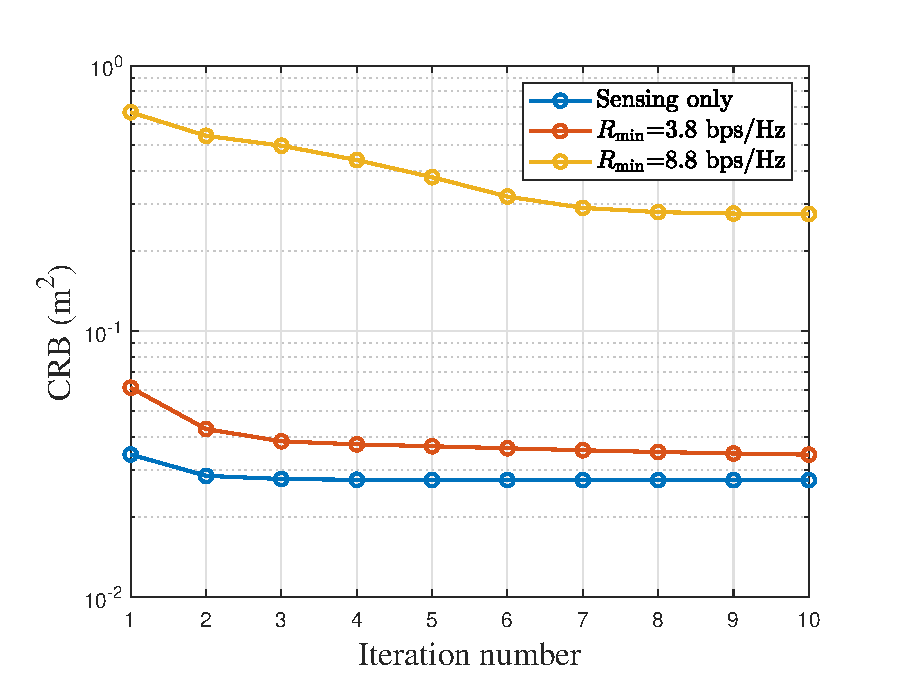
\includegraphics[width=\linewidth]{figure/1_figConv.eps}
    \caption{Convergence behavior of the proposed optimization method}
    \label{fig:Conv}
  \end{minipage}
  \hfill
  \begin{minipage}{0.3\textwidth}
    \centering
    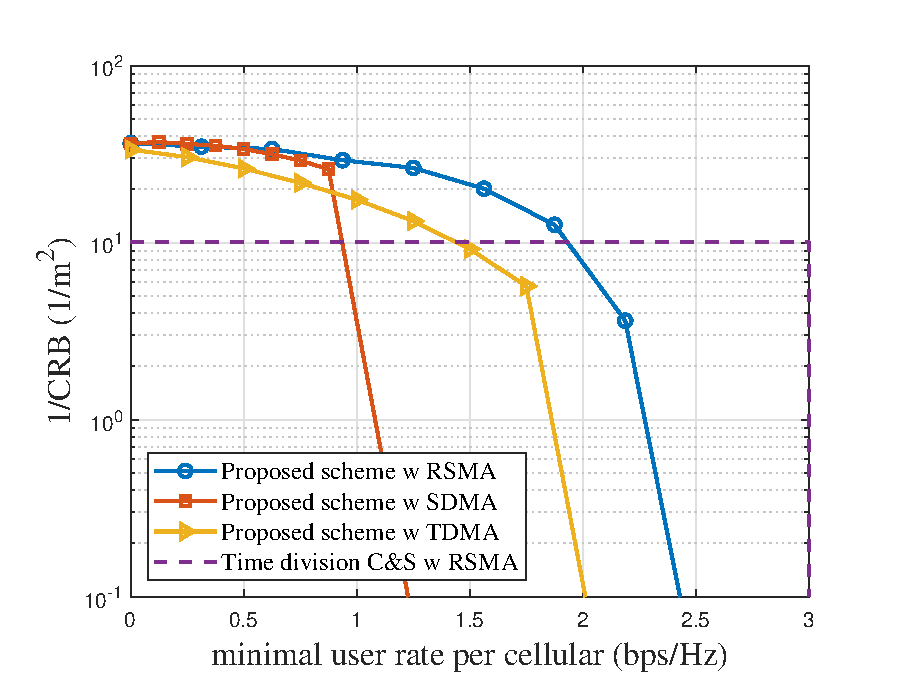
\includegraphics[width=\linewidth]{figure/2_figRate_CRB.eps}
    \caption{Comparison of CRB under different rate constraint}
    \label{fig:image2}
  \end{minipage}
%   \hfill
%   \begin{minipage}{0.3\textwidth}
%     \centering
%     \includegraphics[width=\linewidth]{image3.jpg}
%     \caption{图3标题}
%     \label{fig:image3}
%   \end{minipage}
\end{figure*}
\section{Numerical Simulations}

\printbibliography 
\end{document}


